\chapter{Chapter 2 Title}

\begin{chapterabstract}
Chapter 2 Abstract: Code and figure example.
\end{chapterabstract}

\section{Example Section}

\subsection{Code Example}
Check on conventions on inputting code just to be safe.
This is likely field dependent, so this is worth considering. 
This is the default style, which is aberrant to look at.
In any case, this is how subimport works for nested files to organize your document with each chapter self contained in it's own folder.

\subimport{chap_2_subfiles/}{code}

\subsection{Subfigure Example.}
This is a true subfigure example.
\begin{figure}[h]
    \begin{subfigure}{.55\textwidth}
      \centering
      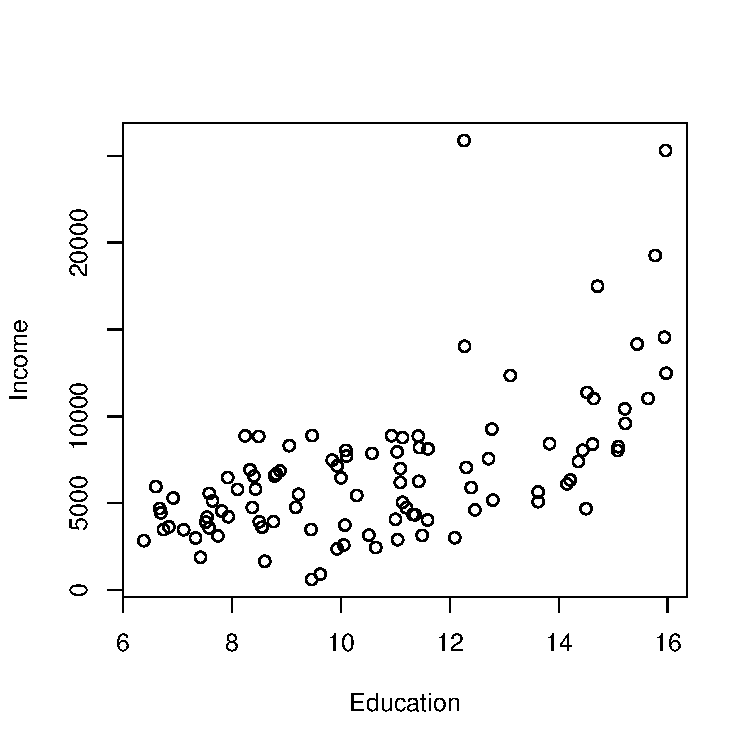
\includegraphics[width=.8\linewidth]{chap_2_figures/example_1}
      \caption{Caption A}
      \label{fig:third_fig_1}
    \end{subfigure}
    \begin{subfigure}{.55\textwidth}
      \centering
      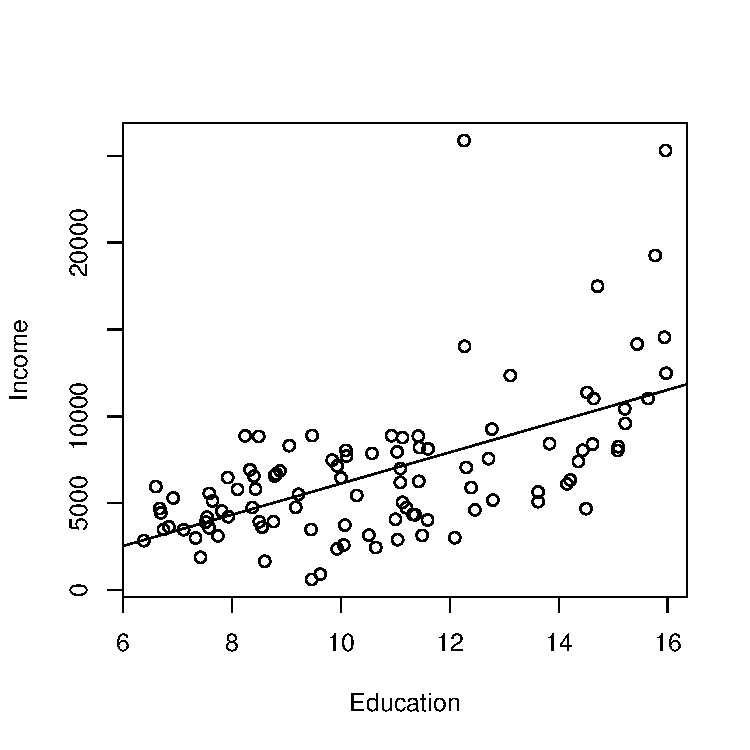
\includegraphics[width=.8\linewidth]{chap_2_figures/example_2}
      \caption{Caption B}
      \label{fig:third_fig_2}
    \end{subfigure}
\end{figure}